\section{Fresnel Style Vocabulary}
\label{fsStyle}

Fresnel lenses specify what information to display but do not give any indication about how to display it. The representation of selected information items mainly depends on the browser's representation paradigm (e.g. nested box layout, table layout, node-link diagrams, advanced widget-based UI, etc.) which defines a default rendering method. The final rendering can however be customized by associating specific styling and layout instructions to elements of the representation, as CSS styling rules do for elements of HTML documents.

Fresnel styling rules are made of a selector and a set of associated styling instructions. Following the lens approach, property \rdf{fresnel:styleDomain} takes a selector as its value (see section \ref{selectors}) and is used to declare the set of RDF properties or resources to which styling instructions apply. Styling instructions themselves are expressed using either Fresnel constructs for RDF-specific styling concepts, or existing languages (CSS \cite{CSS} and SVG \cite{SVG}) for fonts, colors, margins, and borders. 

\subsection{Fresnel Styling Instructions}

Fresnel styling instructions are expressed in RDF and can be used to specify RDF-specific styling concepts such as how properties are labeled and grouped. Fresnel's default behavior is to label properties using the declared \rdf{rdfs:label} of the property type. If this information is not available, then the property's URI is displayed instead. This behavior can be customized thanks to property \rdf{fresnel:label}, which defines whether a property label is displayed (\rdf{fresnel:show}) or not (\rdf{fresnel:none}, see figure \ref{styleCode}), or if it has a fixed custom literal value.

The presentation of property values can also be customized. Fresnel's default property value display method consists in searching for a lens matching the value's type and characterized by purpose \rdf{fresnel:labelLens}. Some kinds of values are however better represented by other means than labels, and it is therefore desirable to specify alternate behaviors. Instruction \rdf{fresnel:value} can be associated with different Fresnel behaviors, such as \rdf{fresnel:image} (see figure \ref{styleCode}) which states that the value to be represented is a URI reference identifying a bitmap image  whose content should be fetched over the Web in order to be displayed. Property values can be grouped, and additional content such as commas and an ending period can be specified using instructions \rdf{fresnel:contentAfter} and \rdf{fresnel:contentLast} to present multi-valued properties. Instruction \rdf{fresnel: contentNoValue} can be used to generate fixed content signaling missing values.

\subsection{CSS and SVG Styling Instructions}

As the set of display elements and layout method depend entirely on the browser's representation paradigm, Fresnel only defines an abstract representation model that can be interpreted and instantiated differently by every application. This abstract model is used to identify the elements of the output document to which CSS and SVG styling instructions can be hooked in a cross-application and cross-format manner. In the abstract model, the container box is the outermost Fresnel container. It identifies the region of the display that contains a group of principal resources to be presented. The container box contains resource and property boxes which identify regions of the display that are respectively associated with resources themselves and their properties. Property boxes are further decomposed as a label box and one or more value boxes which respectively hold the property's label and its value(s). Styling instructions can then be hooked to these presentation elements. The instructions are specified as literal values of properties \rdf{fresnel:containerStyle}, \rdf{resourceStyle}, \rdf{propertyStyle}, \rdf{labelStyle} and \rdf{valueStyle}. Such literal values can contain either styling instructions directly (see figure \ref{styleCode}), or a CSS class name referencing a rule in an external stylesheet.

\begin{figure}
    \begin{center}
      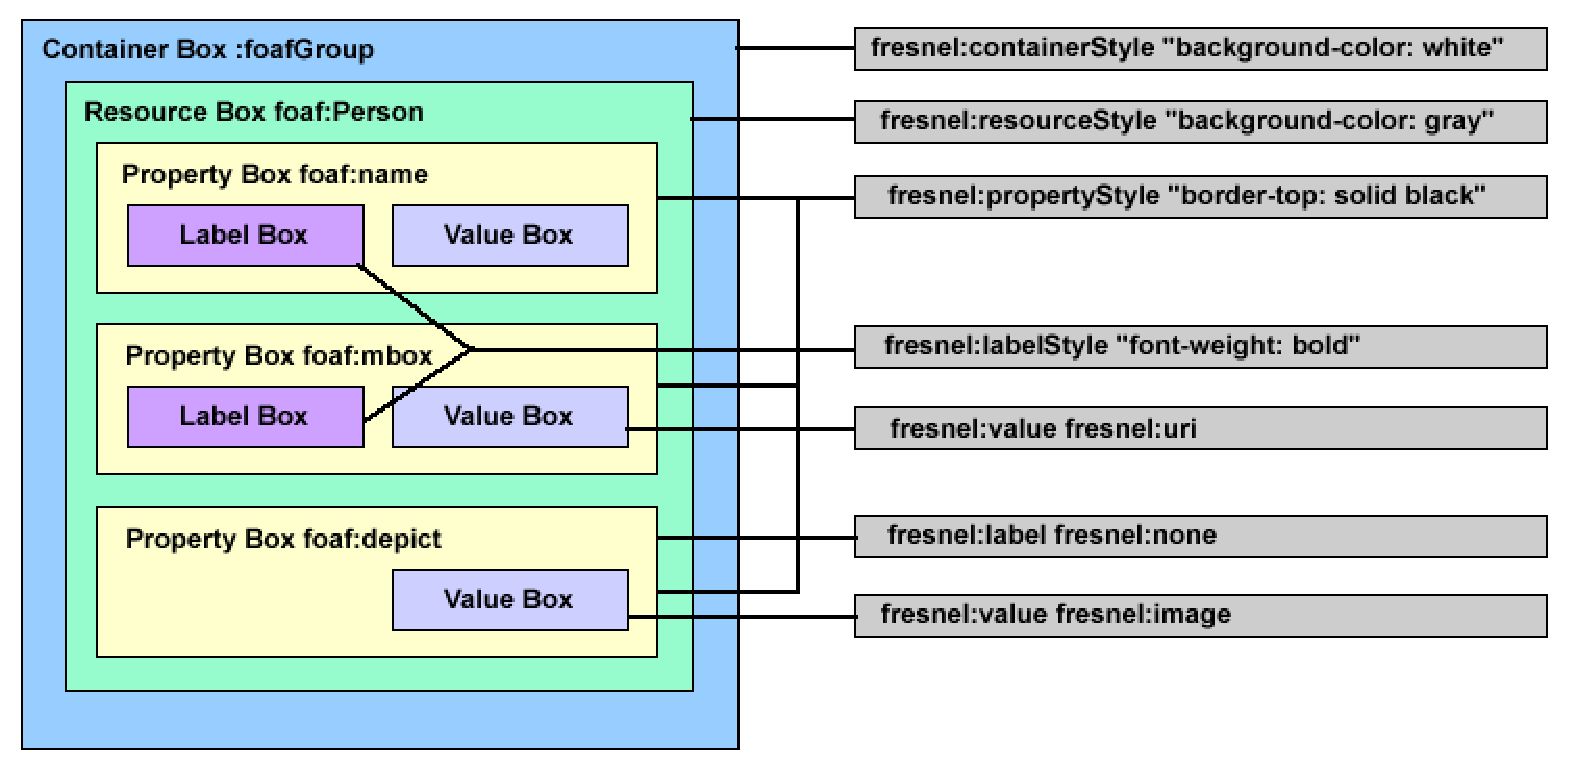
\includegraphics[width=10cm]{boxmodelexample.pdf}
    \end{center}
    \vspace{-0.3cm}
    \caption{Box model with attached styling instructions}
    \label{boxModel}
\end{figure}

Figure \ref{boxModel} contains a schematic view of how the abstract Fresnel model could be interpreted and instantiated by a Web-based browser using the nested box representation paradigm. 

\begin{figure}
    \begin{tabular}{c|c}
      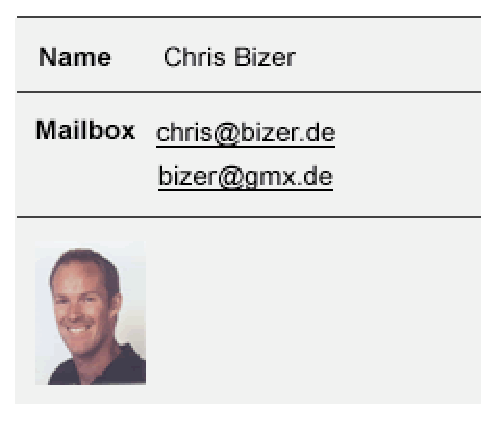
\includegraphics[height=4.3cm]{boxmodelexampleoutput.pdf} &
      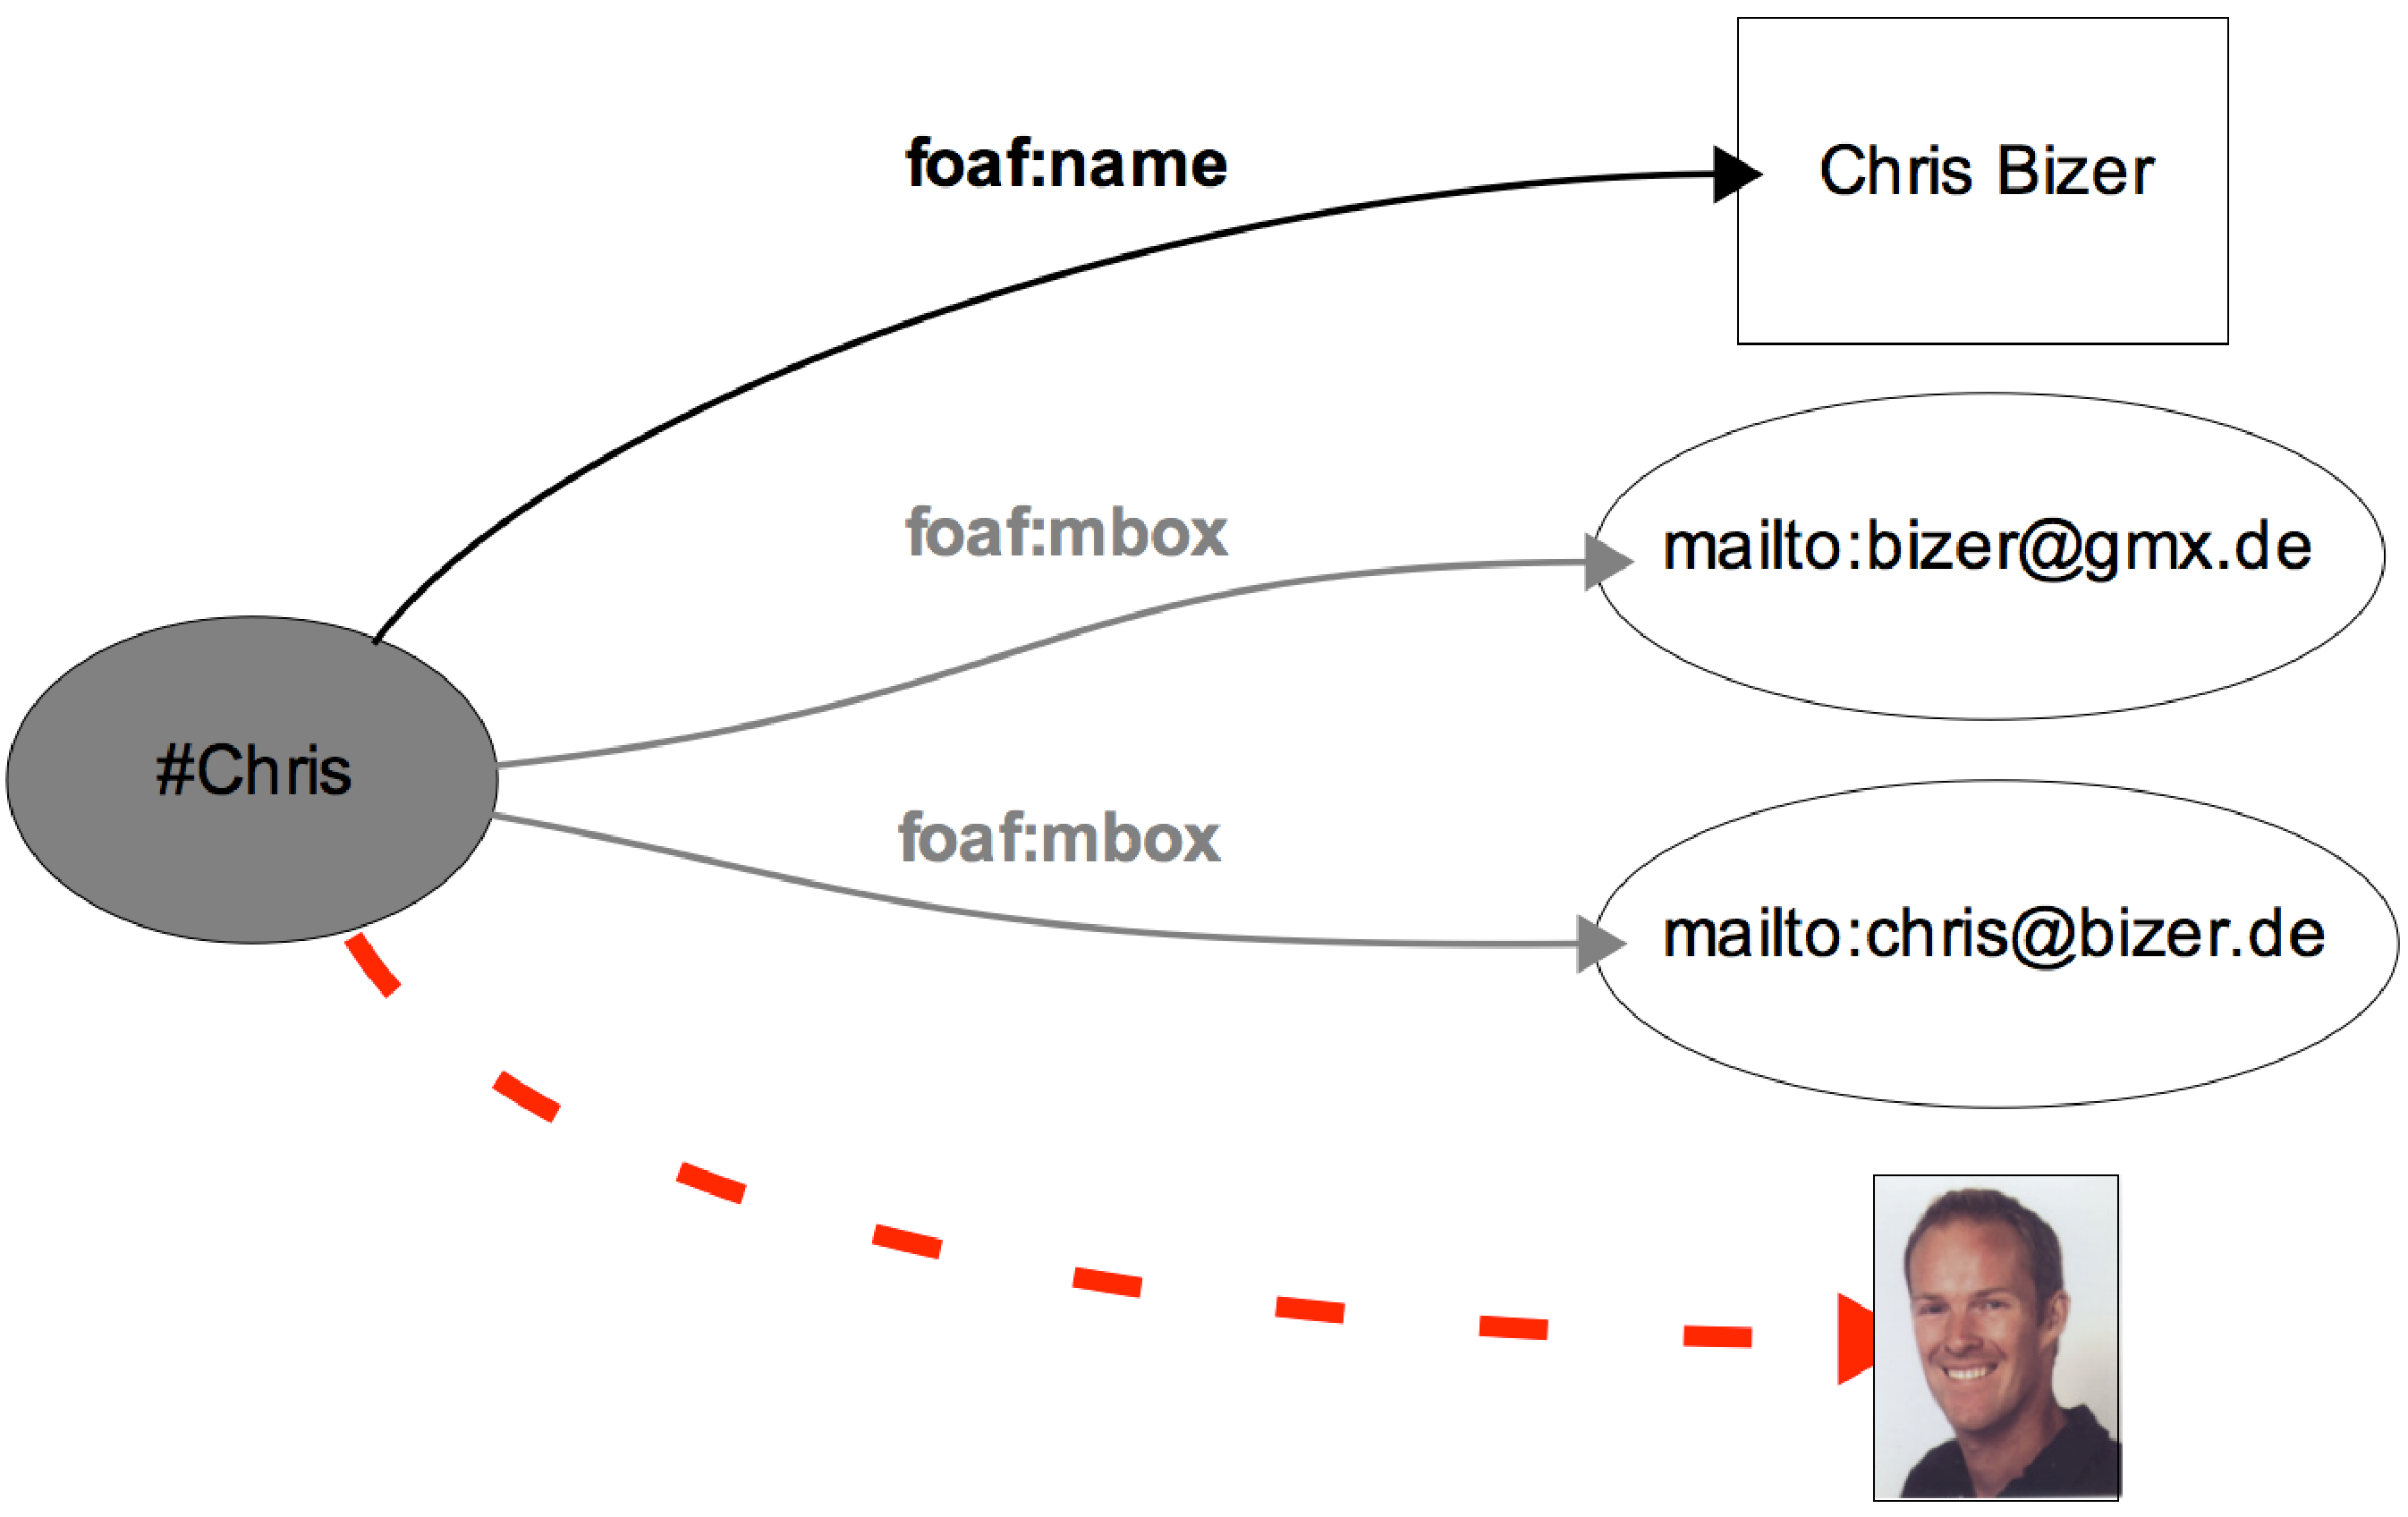
\includegraphics[height=4.3cm]{isv_scs.pdf} \\
      (a) & (b)\\
    \end{tabular}
    \caption{Two interpretations for two representation paradigms}
    \label{boxEx}
\end{figure}

Figure \ref{boxEx}-a shows a possible final rendering based on this model as it might be generated by Longwell. Note that the example model of figure \ref{boxModel} is just one possible instantiation of the abstract Fresnel model. The abstract presentation elements introduced above could be mapped to (possibly non-rectangular) shapes laid out in very different manners, depending on the browser's capabilities and fundamental representation paradigm.

Figure \ref{boxEx}-b shows a different final rendering produced by IsaViz\footnote{This Fresnel presentation was simulated with a GSS stylesheet \cite{Pietriga03} as IsaViz does not support all Fresnel features at the time of submission.}, based on another instantiation of the Fresnel abstract representation model relying on node-link diagrams. The two examples of figure \ref{boxEx} thus illustrate two presentations, by two browsers based on different representation paradigms, of the same data using the same Fresnel lens and styling instructions. But other representation models based on  other paradigms are possible. For instance, a server producing HTML pages for user agents that do not support CSS might choose a basic table-based representation of RDF triples and interpret the property and value boxes as cells of a table row.


The style example of figure \ref{styleCode} specifies that \rdf{foaf:depiction} property values should be displayed as images with a black border, but no property label. Additional styling instructions are used to further customize \rdf{foaf:depiction} properties' appearance. Some of these instructions might be ignored by browsers depending on their relevance with respect to the underlying representation para\-digm. For instance, the border-top instruction will be interpreted by browsers based on a standard box model, whereas it is likely to be ignored by visualization tools such as IsaViz which is more likely to interpret stroke-related instructions.

\vspace{-0.5cm}

\begin{figure}
\begin{small}
\begin{verbatim}
:depictStyle rdf:type fresnel:Style ;
    fresnel:styleDomain foaf:depiction ;
    fresnel:label fresnel:none ;
    fresnel:value fresnel:image ;
    fresnel:propertyStyle "border-top: solid 
                           black"^^fresnel:StylingInstructions;
    fresnel:labelStyle "stroke-dasharray: 10px,20px; stroke-width: 2px; 
                        stroke: red"^^fresnel:StylingInstructions ;
    fresnel:valueStyle "border: solid black"^^fresnel:StylingInstructions.
\end{verbatim}
\end{small}
\vspace{-0.3cm}
\caption{Fresnel style for property \rdf{foaf:depiction}}
\label{styleCode}
\end{figure}

